\documentclass[10pt, a4paper]{article}

% formating packages
\usepackage[a4paper, margin=1cm, bmargin=2cm]{geometry}
\usepackage{titling}

% bibliography packages
\usepackage[backend=biber]{biblatex}

% graphics packages
\usepackage{graphicx}

\graphicspath{ {./plots/} }

% reduce title size by 1cm
\setlength{\droptitle}{-1.5cm}

% set paragraph indent to 0 and paragraph seperation to 5pt
\setlength{\parindent}{0pt}
\setlength{\parskip}{5pt}

% bibliography options
\addbibresource{ref.bib} % Entries are in the ref.bib file

% macros
\newcommand{\pthread}{\textit{POSIX} threads}
\newcommand{\cilk}{\textit{OpenCilk}}
\newcommand{\omp}{\textit{OpenMP}}
\newcommand{\C}{\textit{C}}

\begin{document}

\title{
	\textbf{Parallel \& Distributed Computer Systems}\\
	Exercise 1 -- \textit{Parallel SCC Algorithm}
}
\author{\textit{Alexandros Athanasiadis} -- 10006}
\date{\today}

\maketitle

\begin{abstract}
	\noindent
	This report will showcase my implementation of the SCC coloring algorithm,
	how and where the algorithm was parallelized and the parallel implementations 
	for shared memory systems using \pthread, \omp \ and \cilk. Various figures will compare the 
	serial and parallel implementations, showcasing in which situations the 
	parallel algorithms perform better than serial and by how much.
\end{abstract}

\section{The Algorithm} \label{algorithm}
The Algorithm used is a modified version of `\textbf{Algorithm 2}' from \cite{slota2014}, which
is the `Coloring Algorithm'. The modifications are the ones present in the Assignment document 
(see \ref{coloring}). 

For the implementation I used the Programming Language \C. This came with its own unique challenges when
it came to importing the data given, as the libraries for working with `.mtx' files are somewhat rudimentary. 
The data structure used to store the graph's matrix and the procedure for importing `.mtx' files is described in
\ref{data}

\subsection{The Data Structure} \label{data}
The graphs are given in the `MatrixMarket' file format. The file header contain information about the type
and size of the matrix contained. This information is obtained using the `mmio.h` library which
can be found in the `external' directory. The library and relevant documentation can be found
at \url{https://math.nist.gov/MatrixMarket/mmio-c.html}.

After reading the header information, the rest of the file contains lines of the format:
\begin{verbatim}
row col data
\end{verbatim}
which describe the Adjacency Matrix of the graph using the COO format. For my implementation
I decided to use the Compressed Sparse Row (CSR) and Compressed Sparse Column (CSC) formats, which
have certain advantages when it comes to finding the neighbouring nodes for a given vertex. 

In order to convert from COO to CSR (and the proccess is similar for CSC), first we must sort the
COO entries based on their row indices. Then the column indices in the CSR format is exactly the same
as the COO column indices. For the row indices we store an array such that the array at index $i$ contains
the number of COO entries with row value $i$. Then the CSR row indices is simply the cumulative sum of this
array.

With the CSR data structure the act of getting the vertices that a vertex $v$ points to is as simple as
getting the values of the column index that are between the row indices at $v$ and $v+1$. These vertices
will be referred to as the vertex' neighbours. Equivalently, using the CSC data structure we can get the
vertices that point to the vertex $v$. These will be referred to as the vertex' predecessors.

In addition to these arrays, an array called $is\_vertex$ is stored, which at index $i$ contains `true'
if the vertex $i$ is an active vertex, and `false' if it is not. Then we can remove a vertex from the 
graph by setting its $is\_vertex$ value to `false'.

\subsection{Trimming}	\label{trimming}
Trimming refers to the process of removing the trivial SCCs of the graph, meaning the vertices with in-degree
or out-degree 0. This is a simple process that speeds up the rest of the algorithm significantly.

The trimming procedure is as follows:
\begin{enumerate}
	\item Loop over all vertices $v$ in the graph
	\item Get all neighbours and predecessors of $v$
	\item If the number of neighbours or predecessors is equal to 0, remove the vertex
	\item If the number of neighbours or predecessors is equal to 1 \\
				and the neighbour/predecessor of the vertex is itself, remove the vertex
	\item Repeat until no vertices removed.
\end{enumerate}

The last step's purpose is that removing a vertex may cause another one to become trivial. In reality,
the loop is run a finite number of times (2 in my implementation). This is because each subsequent loop
yields diminishing returns when it comes to time saved, which if overdone ends up making the algorithm
over-all slower.

\subsection{Coloring} \label{coloring}
The coloring step is very similar to \cite{slota2014}, the difference being that the vertices are 
examined ``back to front'', meaning that when we loop over all the vertices $v$, we get all the predecessors $u$
of $v$, and we set $colors[v]$ to be the minimum of $colors[u]$. This is advantageous when it comes to 
parallelizing the algorithm, since we can easily seperate the positions in the $colors$ array where each 
thread can write to (and thus no need for MUTEX).

\subsection{BFS} \label{bfs}
The unique colors are all the indices $c$ in $colors$ such that $colors[c] = c$. Looping over $colors$ we
add these to a temporary stack. Then since each unique color refers to an isolated subgraph of the graph, 
we perform a backwards BFS of that subgraph starting at vertex $c$ and we set the SCC id for each returned
vertex to be equal to $c$. We then remove these vertices from the graph.

\section{Making it Parallel}
The parallelization of the Algorithm described in (\ref{algorithm}) is fairly easy. Each step in the process
can be parallelized with only minor changes. 

The general strategy I employed is one of top-level parallelization, meaning to seperate the large
outer loops between threads and not worry about making the individual methods run in parallel. The reason
I chose this method of parallelization is that the number of threads we can effectively use in an ordinary 
computer is much smaller than the size of the data given and the code is simpler to write and easier to 
understand.

The initialization of the $is\_vertex$ and $colors$ arrays, as well as the coloring loop can be easily 
partitioned into seperate subproblems, with the work shared equally between all threads. Each thread will 
only write to the memory locations that it is assigned to, and so we can avoid race conditions without using
MUTEX locks. 

the trimming and BFS steps need to keep a count of how many vertices were removed and how many sccs were found
in each thread. After all the threads are joined in the main thread, these counts will be summed and then 
used to update the appropriate values accordingly. This is done to avoid using MUTEXes and saves a lot of time.

in finding the unique colors, we need to use a MUTEX when pushing to the stack. This is acceptable since
only a small subset of colors are unique, so the mutex has only a small chance of causing a serialization issue.

\subsection{Implementation with POSIX threads}
The \textit{pthreads} implementation is very straighforward. For each loop we create $num\_threads$ threads. 
We give each thread an equal portion of the indices to process serially, and then let it run until it 
has finished.  Then in the main thread we join the other threads and perform the updates to the global 
variables required.

\subsection{Implementation with OpenMP}
As for \omp, the loops are parallelized using 
\begin{verbatim}
#pragma omp parallel for
\end{verbatim}
statements. The counters for the number of SCCs and the number of removed vertices can be implemented using
\omp \ reducers using the `+' reduce function, while the MUTEX is implemented by using a critical section when
pushing to stack.

\subsection{Implementation with OpenCilk}
The \cilk \ implementation is very similar to the \omp \ implementation, using $cilk\_for$ and $cilk\_reducer$, 
while differing in only 2 steps.

\begin{enumerate}
	\item The loop to find unique colors is not done in parallel. this is due to the lack of MUTEX locks
		in \cilk, which while not changing the result of the program ended up hurting its performance.
	\item An additional reducer (using the or operator) is used in the coloring step, for the boolean tracking 
		if any vertex color has changed. Without this reducer a race condition happened which would terminate
		the loop early, before the color propagation was done.
\end{enumerate}

\section{Results}

We can test the correctness of the implementation by running the serial algorithm for all the example matrices
and compare with the given number of SCCs.

below is sample output from a test script I wrote:
\begin{verbatim}
matrix file        nthd  implem.   n_verts   n_edges   n_sccs    tot_time
==========================================================================
celegansneural      -    SERIAL    297       2345      57        0.000033
foldoc              -    SERIAL    13356     120238    71        0.001220
language            -    SERIAL    399130    1216334   2456      0.984748
eu-2005             -    SERIAL    862664    19235140  90768     2.959949
wiki-topcats        -    SERIAL    1791489   28511807  1         23.017762
sx-stackoverflow    -    SERIAL    2601977   36233450  953658    16.009078
wikipedia-20060925  -    SERIAL    2983494   37269096  975731    34.077497
wikipedia-20061104  -    SERIAL    3148440   39383235  1040035   31.995370
wikipedia-20070206  -    SERIAL    3566907   45030389  1203340   39.983680
\end{verbatim}

The data all seems to match the given information. Running the same script using the other
implementations yields the same results, furthermore by default the program checks if the SCC ids
of each implementation are matching one-by-one. By running the program on all the matrix files I had the
memory and time to check I got matching results every time.

By measuring the time it takes to execute the function, we can get an idea about the performance of the 
different implementations. In Figure \ref{vertices}. we can see the elapsed time as a function of the 
number of vertices for the various example matrices (using 4 threads).

\begin{figure}[h]
	\centering
	\caption{Elapsed Time -- Number of Vertices/Edges}
	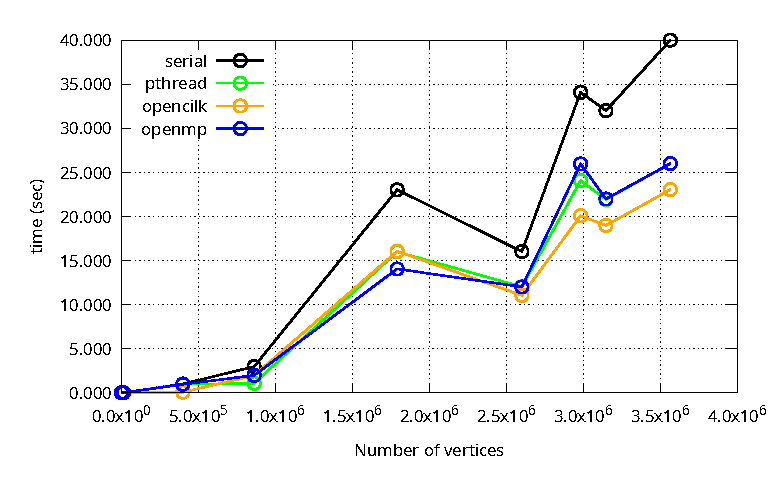
\includegraphics[width=0.45\textwidth]{vertices}
	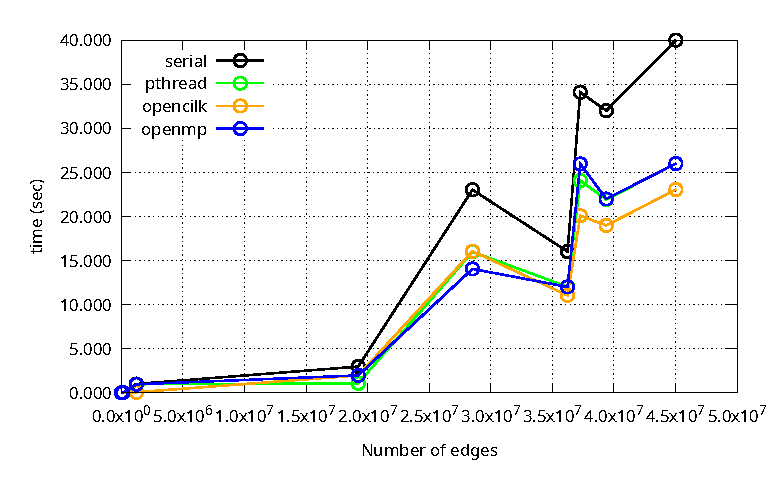
\includegraphics[width=0.45\textwidth]{edges}
	\label{vertices}
\end{figure}

In this example we see how the parallel implementations are faster relative to serial (50-100\% speedup). 
As for which implementation is the best, it varies from graph to graph but \cilk \ is consistently good.

In Figure \ref{threads}. we can see the elapsed time versus the number of threads used (for matrix file 
`wikipedia-20070206'). The optimal amount of threads varies for each implementation, but once again
\cilk \ seems to be the better option using 4 threads (for this graph).

\begin{figure}[h]
	\centering
	\caption{Elapsed Time -- Number of threads}
	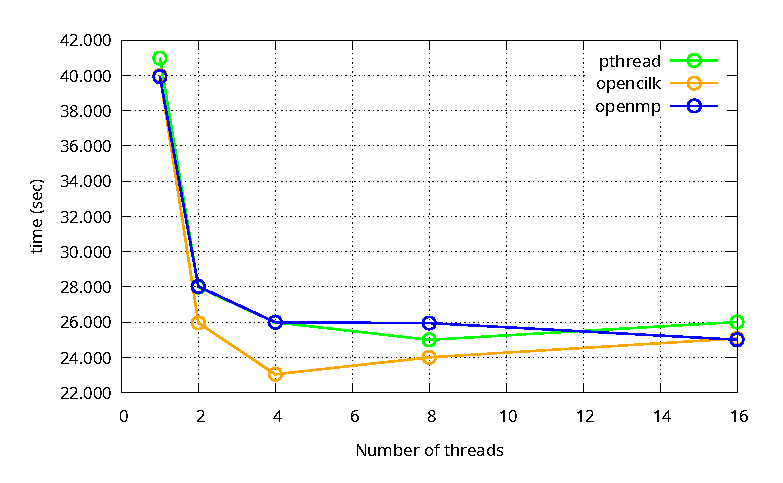
\includegraphics[width=0.45\textwidth]{threads}
	\label{threads}
\end{figure}

\section{Verdict}

With this I would say that this Exercise has yielded the expected/desired results, meaning that the parallel
implementation shows a significant speedup when compared to serial. 

However, I cannot say I am completely satisfied with my results. Even with the parallelization the time it 
takes to run the algorithm is much greater that I would like.

Furthermore, starting with the graph `wb-edu' the time abruptly spikes
to around 23 minutes (serial), and I could not figure out how or why.

Finally my data structure is not very memory efficient. By storing both the CSC and CSR formats 
we effectively double the needed memory to store the matrix. This saves some time in trimming but there may
be a smarter way to handle this.

\printbibliography

\end{document}
